\documentclass[a4paper, 12pt, oneside]{book}
\usepackage{style}

\title{\thesisTitle{}}
\date{\today{}}
\author{Aaron Power}

\makeatletter
\def\@@acrodef{\@ifstar\@acrodefs\@acrodef}
\newtoks\acro@list
\newcommand{\@acrodef}[2]{%
  \global\acro@list=\expandafter{\the\acro@list\@elt{#1}{#2}}%
  \global\@namedef{acro@#1}{n{#1}{#2}}}
\newtoks\acro@resetlist
\newcommand{\@acrodefs}[2]{%
  \global\acro@resetlist=\expandafter{\the\acro@resetlist\@elt{#1}}%
  \@acrodef{#1}{#2}}
\def\acro@doresetlist{\begingroup
  \def\@elt##1{\expandafter\expandafter\expandafter
    \acro@reset\csname acro@##1\endcsname}\the\acro@resetlist\endgroup}
\def\acro@reset#1#2#3{\global\@namedef{acro@#2}{n{#2}{#3}}}
\newcommand{\acro}[1]{\expandafter\expandafter\expandafter
  \use@acro\csname acro@#1\endcsname}
\def\use@acro#1#2#3{\ifx n#1
  #3 (#2)\global\@namedef{acro@#2}{o{#2}{#3}}%
  \else
  #2%
\fi}
\newcommand{\listofacronyms}[1][tabular]{%
  \begingroup\def\@elt##1##2{##1&##2\\}%
  \@ifundefined{chapter}{\section*}{\chapter*}{\listacronymname}
  \noindent\begin{#1}{@{}p{6em}p{\dimexpr\columnwidth-2\tabcolsep-6em\relax}@{}}
    \the\acro@list
  \end{#1}\endgroup}
\providecommand\listacronymname{List of abbreviations}
\newenvironment{acronyms}{\let\acrodef\@@acrodef}{}
\newenvironment{acronyms*}{\let\acrodef\@@acrodef}{\listofacronyms}
\def\g@preto@macro#1#2{\toks0=\expandafter{#1}%
  \toks2={#2}\xdef#1{\the\toks2 \the\toks0 }}
\@ifundefined{chapter}
  {\g@preto@macro\section\acro@doresetlist}
  {\g@preto@macro\chapter\acro@doresetlist}
\makeatother

\begin{document}
  \begin{acronyms}
    \acrodef*{AST}{Abstract Syntax Tree}
    \acrodef*{CMS}{Content Management Systems}
    \acrodef*{CSS}{Cascading StyleSheet}
    \acrodef*{FFI}{Foreign Function Interface}
    \acrodef*{HTML}{HyperText Markup Language}
    \acrodef*{JSON}{JavaScript Object Notation}
    \acrodef*{I18n}{Internationalization and localization}
    \acrodef*{XSLT}{Extensible Stylesheet Language Transformations}
    \acrodef*{XML}{Extensible Markup Language}
  \end{acronyms}
  \maketitle
  \chapter*{Abstract}
  \addcontentsline{toc}{chapter}{Abstract}
  This thesis describes the process of building a templating language in Rust. Using various sources such as \textit{``Compilers: Principles, Techniques, and Tools''} to build a compiler, and have it interact with Rust. This thesis also addresses the problems of existing templating languages, and how \languageName{} attempts to solve.
   \chapter*{Declaration}
  \addcontentsline{toc}{chapter}{Declaration}
  The incorporation of material without formal and proper acknowledgment (even with no deliberate intent to cheat) can constitute plagiarism.
  If you have received significant help with a solution from one or more colleagues, you should document this in your submitted work and if you have any doubt as to what level of discussion/collaboration is acceptable, you should consult your lecturer or the Course Director.\\
  \textbf{WARNING:} Take care when discarding program listings lest they be copied by someone else, which may well bring you under suspicion. Do not to leave copies of your own files on a hard disk where they can be accessed by other. Be aware that removable media, used to transfer work, may also be removed and/or copied by others if left unattended. Plagiarism is considered to be an act of fraudulence and an offence against Institute discipline.
  Alleged plagiarism will be investigated and dealt with appropriately by the Institute. Please refer to the Institute Handbook for further details of penalties. The following is an extract from the B.Sc. in Computing (Hons) course handbook. Please read carefully and sign the declaration below
  Collusion may be defined as more than one person working on an individual assessment. This would include jointly developed solutions as well as one individual giving a solution to another who then makes some changes and hands it up as their own work. Failure to complete and submit this form may lead to an investigation into your work.
  \textbf{DECLARATION:} 
  I am aware of the Institute's policy on plagiarism and certify that this thesis is my own work.\\
  Student:\_\_\_\_\_\_\_\_\_\_\_\_\_\_\_\_\_\_\_\_\_\_\_\_\_\_\_\_\_\_\_\_\_\_\_\_\_\_\_\_\_\_\_\_\_\_\_\_\_\_\_\_\_\_\_\_\_\_\_\_\_\_\_\_\\
  Signed:\_\_\_\_\_\_\_\_\_\_\_\_\_\_\_\_\_\_\_\_\_\_\_\_\_\_\_\_\_\_\_\_\_\_\_\_\_\_\_\_\_\_\_\_\_\_\_\_\_\_\_\_\_\_\_\_\_\_\_\_\_\_\_\_\_
  \chapter*{Acknowledgments}
  \addcontentsline{toc}{chapter}{Acknowledgments}
  I would like to thank my project tutor John Montayne, for his guidance throughout the project. I would also like to thank everyone in the Rust community for helping me figure out Rust, and problems I had with my code.
  \tableofcontents
  \listoffigures
  \listofacronyms
  \chapter{Background Research}
  \chapter{Background Research}
\section{Introduction}

A \compiler{}  is a compiler that converts source code into some other form of source code, as opposed to a traditional compiler which converts human readable source code into machine instructions. This has a wide array of uses within different implementations. CMS'(Content Management Systems) have templates that writers pass in their writing to format it into a HTML article on their Website. Academics use \LaTeX{} to convert plain text into scientific documents, and reports. Their use in this thesis is to create a templating language which is a programming language that will convert it's source code into HTML for use in Web applications. The purpose of \languageName{} is to create a templating language that Web developers can use to have more modular, and scalable markup in their Web application.

While there is no definitive first templating language. Their popularity began around the late 1990's with XSLT(Extensible Stylesheet Language Transformations) in 1999 in a W3C recommendation document \parencite{XSLT}. Which was designed for transforming XML(Extensible Markup Language) documents into other formats IE: PDF's as shown in \parencite{XSLTEx}.
\newpage 

One of the most popular modern templating languages for use within Web applications is \parencite{Mustache}. Mustache is a ``\textit{logic-less}'' templating language, meaning it has no explicit control flow statements \textit{if, else, for} according to the \parencite{MustacheMan}. Everything is instead based on the object that is passed to the template See Figure ~\ref{fig:mustacheEx}. So if the developer couldn't change the markup if someone's name started with A instead of B unless they add a key to the hash before they pass it to the Mustache templating engine. Mustache is not a HTML specific templating language. Meaning it's syntax is completely independent from it and can be used with anything. However this also means it as language can't use assumptions based on the language leading the syntax to be very verbose. 

\begin{figure}[ht!]
    \small
    \setstretch{1.0}
    \begin{verbatim}
            A typical Mustache template:

                Hello {{name}}
                You have just won {{value}} dollars!
                {{#in_ca}}
                Well, {{taxed_value}} dollars, after taxes.
                {{/in_ca}}

            Given the following hash:

                {
                  "name": "Chris",
                  "value": 10000,
                  "taxed_value": 10000 - (10000 * 0.4),
                  "in_ca": true
                }

            Will produce the following:

                Hello Chris
                You have just won 10000 dollars!
                Well, 6000.0 dollars, after taxes.
    \end{verbatim}
    \caption{A Mustache Example, from \parencite{MustacheMan}}
    \label{fig:mustacheEx}
\end{figure}
\clearpage



\section{Advantages of a templating language in the Web.}
As the Web has advanced there has always been a need to be able to have the document delivered to the user to be able to be changed based on who, and how the document is being requested. The most popular way to do this currently is to serve the user a nearly blank HTML(HyperText Markup Language) document containing links to JavaScript files that once downloaded, and executed will fill the DOM(Document Object Model) with the data, and information based on the user's request. Prime examples of this is JavaScript frameworks like React. In which the standard is to have a HTML document with a single \textcolor{red}{<div>} element, and let React build the DOM once it can.

%%%%%%%%%%%%%%%%%%%%%%%%%%%%%%%%%%%%%%%%%%%%%%%%
\begin{figure}[ht!]
    \small
    \setstretch{1.0}
    \begin{verbatim}
        <!DOCTYPE html>
        <html>
            <head>
                <meta charset="UTF-8" />
                <title>Hello React!</title>
                <script src="build/react.js"></script>
                <script src="build/react-dom.js"></script>
                <script src="build/script.js"</script>
            </head>
            <body>
                <div id="example"></div>
            </body>
        </html>
    \end{verbatim}
    \caption{Standard React HTML index file}
\end{figure}
%%%%%%%%%%%%%%%%%%%%%%%%%%%%%%%%%%%%%%%%%%%%%%%%

This comes with problems. The content of the Web page is dependent on the JavaScript. While the JavaScript is being downloaded the user will only see a blank page. This problem becomes especially apparent when the user is on a mobile network, or has a slow connection. Studies have shown that 47\% of mobile users expect a site to load in less than two seconds, that 40\% of mobile users will abandon a site if it doesn't load in three seconds or less, and that 52\% of users said that a quick page load is important to site loyalty according to \parencite{MobileLoad}. In large scale applications, and businesses JavaScript size quickly becomes a huge bottleneck in the load times of Websites as shown by \parencite{VergeJS}.\newline

It is in this area in particular that the advantages of using a templating language is seen. With a templating language the content of the Web page can be sent in the initial HTML page, making the ``perceived'' load time of the Web page very quick. Giving the JavaScript more time download than if the user were to see a blank page.\newline

Having a templating language can also provide good separation between the data model of the language, and the design of the page. The designers, or client-side programmers who are formatting the Web page don't have to worry about how the server-side logic works, or write code that could change server's data-model in order to change the format of the Web page. 
\newpage
\section{Main features of \languageName{}}
From doing my own research and looking at the two comparisons of both templating languages in established server-side programming languages(\textit{PHP, C\#, .NET}) from \parencite{WikiCompare}, and templating languages made specifically for use in Isomorphic JavaScript which are generally much younger in their development than their traditional language equivalents as shown in \parencite{JSCompare}.

From looking at these languages I think the main features of \languageName{} is to first have inheritance, and includes, and variables which is to mean that you can write parent markup files which have child markup files which when parsed will include the markup of the parent, that arbitrary \languageName{} files can be inserted into other \languageName{} files, and be able to have data injected within the template respectively. 

One feature that seems to be most absent, or lacking in strong support in most the languages is I18n(\textit{Internationalization and localization}) support. In the modern Web it seems that having poor I18n support is a huge weakness in a templating language for the Web. According to Alexa estimates Google.com's top five countries are as follows United States, India, Japan, Brazil, and Russia. Out of 5 of the top countries only one of those is an English speaking country, and only two of which are Latin based languages. It is important now more than ever to have strong support for other speaking languages.
\newpage
\section{Building a \compiler{}.}
Building \compiler{} is a difficult task. The two primary sources for building a \compiler{} will be Compilers Principles Techniques and Tools (2nd Edition) by \parencite{DragonBook} also known as ``\textit{The Dragon Book}'', and Parsing Techniques - A Practical Guide (2nd Edition) by \parencite{ParseTech}. Since the project is for a \compiler{}, and not a traditional compiler, there is a lot within the sources that won't be used. For example The Dragon Book has chapter's such as ``Run-Time Environments'', and ``Machine-Independent Optimizations'' which don't relate as are output is HTML, and not Machine Code. The syntax, and the features of the language will need to be mostly finalised early within the project to prevent any sort of feature creep, or spending time, and resources on changing the style of the language. Especially aspects like whether to have natural templates, which are templates which are independent of the language, and have a much more verbose language similar to \parencite{Mustache}, or to have a much more terse language, but have it only work for outputting HTML files, like \parencite{Jade}. 

\section{Why Rust?}
There are many reasons that make Rust an great candidate for building a \compiler{}. Rust doesn't have a garbage collector that other languages like Java, or JavaScript. This reduces the runtime overhead of the program giving a significant performance boost, which is important for doing on request compilation of templates on a server. Rust's \textcolor{blue}{char} type is a Unicode scalar value. Meaning Rust can handle non-Latin characters much more easily than languages without IE: JavaScript. Which would be an important feature since the \languageName{} will have strong I18n support. Since rust has such a minimal runtime, it has strong FFI(Foreign Function Interface) support, meaning the \compiler{} can be used in servers written in different languages, without requiring the compiler to be rewritten in that language, and keeping the performance gains from having it built in Rust.
  \chapter{Literature Review}
  % \chapter{Determining how to parse a formal language}

\section{Introduction}
% About how compilers work, three parts. the lit review focus on parsing part

\newpage
\section{Language Parsing Design}

\subsection{Determining how to parse the syntax of a language}

A formal language is defined as a set of strings of symbols for use in situations where a natural language(\emph{English}) isn't suitable eg. Mathematics, and Computer programming. Where each symbol has precise semantic, and syntactic relation to each other. Writing formal grammar rules uses a set of finite ``\emph{productions}''. Productions, are rules that signify substitution of symbols within a string, there are typically three symbols when writing productions in formal grammars.

\begin{description}
    \item[\emph{Terminal Symbols}] Symbols which cannot be substituted any further, examples of this in programming languages are single number digits(0-9), and matematical symbols(\emph{+,-,/,*}). Terminal symbols are commonly represented by lowercase letters.
    
    \item[\emph{Nonterminal Symbols}] Symbols which can be reduced further using productions. For example as in \ref{fig:formalGrammar} $A \rightarrow a\ |\ aA$ is a nonterminal rule, as \emph{A} needs to be substituted into either \emph{a}, or \emph{aA}. Nonterminal symbols frequently are represented by uppercase letters.

    \item[\emph{Start Symbol}] is a special Nonterminal symbol signifying the start of a string. Start symbols are represented by a uppercase S, or with a Uppercase letter with a subscript s eg. $S_s$, in order to signify it is different from a Nonterminal \emph{S} symbol.
\end{description}


Productions rules are used show how a compiler will take strings, and convert them into tokens. The tokens are sorted into a hierarchy that can be used by the next stage of the compiler. The \emph{|}, known as the vertical bar or ``pipe'' symbol is just used to symbolise a grouping of rules applying to the same rule.

\begin{figure}[ht!]
    \begin{align*}
    S_s &\rightarrow AB\ |\ CC \\
    A &\rightarrow a\ |\ aA \\
    B &\rightarrow bc\ |\ bBc \\
    D &\rightarrow ab\ |\ aDb \\
    C &\rightarrow c\ |\ cC \\
    \end{align*}
    \caption{Formal grammar syntax, example from \autocite{ParseTech}}
    \label{fig:formalGrammar}
\end{figure}

\subsection{Chomsky hierarchy within formal languages}

When parsing a string as a way to meaningfully turn the language into meaningful data models, \autocite{Chomsky} talks about the need of structured models, rather than using probabilistic models like Markov Chain. Markov chain is a model where the data model changes from different states, based solely on it's most recent state. \autocite{Chomsky} showcases this with the famous example: \\\\ \centerline{``\emph{Colorless green ideas sleep furiously}''} \\

A sentence which is not a semantically valid sentence, but is grammatically correct. In \autocite{Chomsky} he defined what is now known as \emph{\hierarchy{}}, which defines formal languages into four types(Type 0 - 4). As shown in Figure \ref{fig:Chomsky} each type is a subset of the previous. All of Type 4, can be a Type 3, but not all of Type 3 can be Type 4, so multiple rules can describe the same language depending on it's syntax.
\clearpage
\begin{figure}[h]
    \centerline{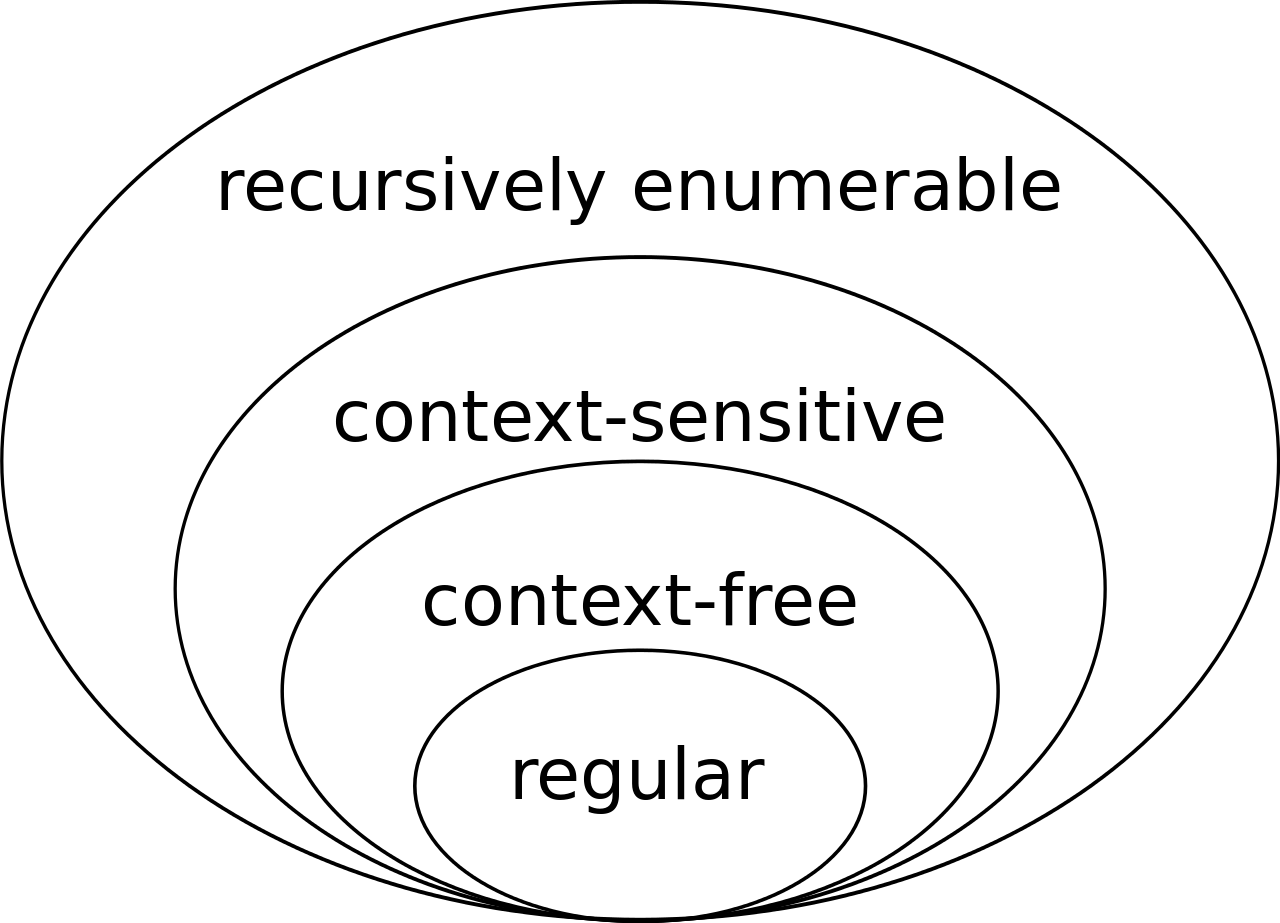
\includegraphics[width=0.5\linewidth]{img/Chomsky.png}}
    \caption{\hierarchy{}, by J. Finkelstein}
    \label{fig:Chomsky}
\end{figure}
\begin{description}
    
    \item[Type 0] Also known as \emph{recursively enumerable} languages. This is the the parent of all following languages. Every language in the Chomsky hierarchy is also a recursively enumerable. Recursively enumerable is a generalised, and can have unclear hierarchy, due to it's lack of limitations.
    
    \item[Type 1] Also known as \emph{context-sensitive} languages. Meaning only one of the nonterminal characters on the left hand side can be replaced. This allows for a much clearer hierarchy within the parse tree.
    
    \item[Type 2] Also known as \emph{context-free} languages. context-free is similar to context sensitive, except there is always only one Nonterminal Symbol on the left hand side. This prevents children in the parse tree to have star patterns with multiple parents pointing to the same child, which then points to multiple children within the parse tree. This is known as a \emph{pure} hierarchy. This is a the language type most programming languages fall under, with few exceptions(\emph{C++}).

    \item[Type 3]  Also known as \emph{regular} languages. Regular languages are languages defined by \emph{regular expressions} rather than regular grammar like seen previously. Regular expressions are often used when the lexical rules of a language are simple, and don't require powerful notations like grammars. Regular expressions are also much more concise in the expressing notation, than it's grammar equivalents. However regular expressions cannot describe nested structures within the language, which can be very limiting \autocite{DragonBook}.
\end{description}

\subsection{Using \hierarchy{} \\within a compiler}
When discussing about parsing a programming language, it is important to differentiate between the syntax of the language, and the \emph{semantics} of the language. As confusion between the two can lead an individual to believe a language is one type, when it is actually a subset. As \autocite{DragonBook} shows, compilers when parsing language have a lexical analyser, which would group characters into much more meaningful sequences known as \emph{lexemes}. Lexemes are then converted into a tokens commonly in the form of a key, value pairing.\\\\ \centerline{(\emph{token-name}, \emph{attribute-value})} \\

Raw symbols like digits, or mathematical symbols(\emph{+,-,/,*}) are mapped into their token-name equivalents. Where as variables, the compiler will map the token-name to a token representing that it is an identifier eg. \emph{id, ident, identifier}. The compiler will then assign the attribute-value to number representing it's key in the Symbol-Table. The Symbol-Table is designed to contain much more concrete information about the token, such as it's name, and it's type eg. \emph{int, float, double, string}. The set of tokens is then passed to the syntax analyser. 

The syntax analyser will only look at the token-name getting only a vary abstract representation of the code, and can only report syntactical errors such as using wrong keywords, or having incorrect mathematically expressions eg $x = 1 + - + 1$. This is shown clearly in Figure \ref{fig:InvalidC}. Where when run through a C compiler the compiler will print out ``\emph{error: \lq{}x\rq{} undeclared (first use in this function)}''. 

\begin{figure}[ht!]
    \begin{verbatim}
                int main() {
                    x++;
                    int x = 1;
                    return 0;
                }
    \end{verbatim}
    \caption{C code with valid syntax, but invalid semantics.}
    \label{fig:InvalidC}
\end{figure}

This could lead an individual that the syntax of the parser, and thus the language must be context-sensitive, as the compiler knew that ``\emph{x}'' was being used before it existed. As seen in \autocite{DragonBook} the compiler could be using a parsing grammar that is context-free, and the semantic analyser is what determined that the code written was invalid. As the syntax analyser goes through each token it builds a parse tree, showing the relationship of the tokens as seen in Figure \ref{fig:AST}. It is solely within the syntax analyser that defines the language type of the programming language.
\begin{figure}[ht!]
    \centering
    \begin{tikzpicture}
        \tikzset{every tree node/.style={align=center,anchor=north}}
        \Tree[.= [.x \textit{id} {} ] 
                 [.+  
                     [.1 ] 
                     [.- {}  
                         [.+ {} 
                             [.1 ] 
                         ] 
                        ]  
                     ]  
                 ]  
             ] 
    \end{tikzpicture}
    \caption{An Abstract Syntax Tree.}
    \label{fig:AST}
\end{figure}

The semantics of the language are typically defined within a semantics analyser. One common part included within the analyser is \emph{type checking}. Where the compiler checks the types on both sides of an operand(\emph{+,-}). An example used in \autocite{DragonBook} is array indexing. As commonly programming languages require the index number to be an integer eg. array[1], not array[1.5].


\autocite{DragonBook} recommends, using a tools like \emph{Lex} for generating code from grammars that were discussed earlier. \autocite{LexYacc} argues that creating parsers like 

\newpage
\section{Conclusion}
\newpage

  \chapter{Practical Guide}
  \section{Introduction}
In this section, the focus will be on constructing \acro{HTML} from Jade, an existing templating language. This example will not cover every feature, or edge case, but will show concisely how a person would build a parser, and how parsing works in practical terms. The Jade that will be converted is the Figure ~\ref{fig:jade}. This will be converted to the code shown in Figure ~\ref{fig:html}, except without the whitespace(except within text), and newlines. The ``->'' character represents the tab character. While Jade can handle tabs or space characters, for simplicity this will focus purely with the tab character. Jade is whitespace sensitive meaning if the the leading whitespace(The whitespace at the start of a line) is more than the previous line, the element on the line is the child of the element from the previous line. The ``.'' syntax as seen in Figure ~\ref{fig:jade}, is shorthand for adding a class to the element so ``\textit{p.article}'' would become ``\textit{<p class=\'article\'></p>}''.

\begin{figure}[ht!]
    \small
    \setstretch{1.0}
    \begin{verbatim}
        html
        ->body
        ->->p.article Hello World!
    \end{verbatim}
    \caption{Sample Jade code to be parsed.}
    \label{fig:jade}
\end{figure}

\begin{figure}[ht!]
    \small
    \setstretch{1.0}
    \begin{verbatim}
        <html>
            <body>
                <p class="article">
                    Hello World!
                </p>
            </body>
        </html>
    \end{verbatim}
    \caption{Sample \acro{HTML} code to be created from Figure ~\ref{fig:jade}.}
    \label{fig:html}
\end{figure}

\section{Definitions}
For this example there will be two main structs(A struct is a basic data structure with fields containing data). The ``\textit{parser}'' struct, and ``\textit{Element}'' struct. Where the parser struct represents the parser itself, and containing methods related to handling the input, and output of the program. Code samples containing method definitions are shorten to signatures for brevity.

\subsection{Element}
The ``\textit{Element}'' struct defines an individual element within both the \acro{AST}, and \acro{HTML}. Markup languages such as \acro{HTML} can usually be translated directly from \acro{AST} representation to code, due to their already present parent-child relation. Features that don't directly translate such as variables, or keywords(extends, includes), it'd be better to have a ``\textit{Node}'' struct, that could contain the either the element struct, or another defining rules of the other features. Both structs also implement the ``\textit{Debug}'' trait to allow them to be easily printed to the console.

\subsubsection{Element Properties}
\begin{itemize}
    \item[\textbf{tag:}] The html tag of the element. eg. \textit{html, body, h1, p}
    \item[\textbf{indentation:}] In Jade leading whitespace defines the hierarchy of the elements. So it is important to keep track of the whitespace.
    \item[\textbf{attributes:}] A Key-Value pairing of the attributes, with the attribute name as the hey, and their value as 
    \item[\textbf{classes:}] The class attribute is the only html attribute that accepts multiple values, so it wouldn't fit within attributes.
    \item[\textbf{text:}] The plain text within the element.
    \item[\textbf{children:}] The child elements of the element.
\end{itemize}

\subsubsection{Element Methods}
\begin{itemize}
    \item[\textbf{new}] Creates, and returns an empty Element.
    \item[\textbf{generate\_html}] Returns a \textit{String} of html code, based on it's properties. This method is also recursive. Calling each of it's children's \textbf{generate\_html} methods.
    \item[\textbf{get \& set}] The get, and set methods for all the properties above.
    \item[\textbf{add \& remove}] For properties containing multiple values like classes, children, and attributes. They would also have methods for pushing, and removing an individual value from them.
\end{itemize}

\begin{figure}[ht!]
    \small
    \setstretch{1.0}
    \begin{verbatim}
      #[derive(Debug)]
      struct Element {
        tag: String,
        indentation: u8,
        classes: Vec<String>,
        attributes: HashMap<String, String>,
        text: String,
        children: Vec<Element>,
      }

      impl Element {
        fn new() -> Self { unimplemented!() }
        fn generate_html(&self) -> String { unimplemented!() }
        fn get_tag(&self) -> String { unimplemented!() }
        fn set_tag(&mut self, tag: String) { unimplemented!() }
        fn get_indentation(&self) -> u8 { unimplemented!() }
        fn set_indentation(&mut self, indentation: u8) 
        { unimplemented!() }
        fn get_classes(&self) -> Vec<String> { unimplemented!() }
        fn set_classes(&mut self) { unimplemented!() }
        fn get_attributes(&self) -> HashMap<String, String> 
        { unimplemented!() }
        fn set_attributes(&mut self) { unimplemented!() }
        fn get_text(&self) -> String { unimplemented!() }
        fn set_text(&mut self, text: String) { unimplemented!() }
        fn get_children(&self) -> Element { unimplemented!() }
        fn set_children(&mut self) { unimplemented!() }
        fn add_child(&mut self, child: Element) { unimplemented!() }
        fn add_attribute(&mut self, key: String, value: String) 
        { unimplemented!() }
        fn add_class(&mut self, class: String) { unimplemented!() }
        fn remove_child(&mut self, child: Element) { unimplemented!() }
        fn remove_attribute(&mut self, key: String) { unimplemented!() }
        fn remove_class(&mut self, class: String) { unimplemented!() }
      }
    \end{verbatim}
    \caption{Element code}
\end{figure}

\subsection{Parser}
The parser struct represents the Parser itself. All logic with regards to moving through the input given by the user is either handled within this struct, or through calling methods on this struct.

\subsubsection{Parser Properties}
\begin{itemize}
    \item[\textbf{input:}] The source code given by the user. Usually the contents of a file.
    \item[\textbf{position:}] The parsers position within the input. 
    \item[\textbf{output:}] A vector of the elements parsed.
\end{itemize}

\subsubsection{Parser Methods}
\begin{itemize}
    
    \item[\textbf{new}] Creates, and returns a new parser containing the source passed in.
    
    \item[\textbf{take}] Returns an Option either containing the next character, and removes it from the input. Or None indicating EOF(End Of File).
    
    \item[\textbf{eof}] checks if we've reached the end of the source.
    
    \item[\textbf{peek}] Returns an Option either containing the next character, but doesn't remove it from the input. Or None indicating EOF.

    \item[\textbf{take\_spaces}] Removes characters until the character isn't whitespace(space, tab, newline, carriage return), and returns how many characters were removed.

    \item[\textbf{take\_until}] Takes, and remove characters from the source until it reaches the character passed as a parameter. Then returns a Result either containing a String of all the characters taken excluding the character passed, or a ParseError indicating that something went wrong while taking the characters. eg. EOF.

    \item[\textbf{peek\_until}] Takes, but doesn't remove characters from the source until it reaches the character passed as a parameter. Then returns a Result either containing a String of all the characters taken excluding the character passed, or a ParseError indicating that something went wrong while taking the characters. eg. EOF.
    
    \item[\textbf{take\_while}] Takes, and removes characters, while the function passed evaluates to false. The function passed in, is passed a char, which is the the latest character in the stream.
    
    \item[\textbf{get \& set}] The get, and set methods for all the properties above.
\end{itemize}

\begin{figure}[ht!]
    \small
    \setstretch{1.0}
  \begin{verbatim}
    #[derive(Debug)]
    enum ParseError {
      EOF,
      EncodingError,
    }
    #[derive(Debug)]
    struct Parser {
      input: String,
      position: usize,
      output: Vec<Element>
    }
    impl Parser {
      fn new(source: String) -> Self { unimplemented!() }
      fn take(&mut self) -> Option<char> { unimplemented!() }
      fn peek(&mut self) -> Option<char> { unimplemented!() }
      fn eof(&self) -> bool { unimplemented!() }
      fn take_spaces(&mut self) -> u8 { unimplemented!() }
      fn take_until(&mut self, character: char) 
      -> Result<String, ParseError> { unimplemented!() }
      fn peek_until(&mut self, character: char) 
      -> Result<String, ParseError> { unimplemented!() }
      fn take_while<F>(&mut self, condition: F) 
      -> Result<String, ParseError> 
        where F : Fn(char) -> bool { unimplemented!() }
      fn get_input(&self) -> String { unimplemented!() }
      fn set_input(&mut self, input: String) { unimplemented!() }
      fn get_position(&self) -> usize { unimplemented!() }
      fn set_position(&mut self, position: usize) { unimplemented!() }
      fn get_output(&self) -> Element { unimplemented!() }
      fn set_output(&mut self, output: Element) { unimplemented!() }
    }
  \end{verbatim}
  \caption{Parser code}
\end{figure}
\newpage
\newpage
\section{Parser Logic}
Once, the program has read the source into memory, and the parser is instantiated the program begins a loop that will run until the end of the source. This loop will contain the logic for parsing. First the program checks if the line is empty or contains all whitespace, if does the program will simply ignore it. Jade is a line sensitive language, so elements can't continue onto the next line without the use of special characters, and their implementation is out of scope for this guide. A new blank element is created, and the parser reads in how many leading spaces on the line in order to determine heirarchy, the heirarchy is defined once every element has been parsed, for simplicity. The program runs the the \textbf{take\_while}, with a closure, that evaluates based on whether the character is a ``\textit{.}'', ``\textit{\#}'', ``\textit{(}'' symbols, or if it is whitespace. For example with the line ``\textit{article.class}'' take\_while will pull out the ``article'', and place that as the element's tag. The program then begins another while loop that continues until the end of the line. Matching for the symbols mentioning before, with ``\#'' meaning id, ``.'' meaning class, ``('' meaning atrributes eg. ``(href=\textquotedbl{}\#\textquotedbl{} required=\textquotedbl{}true\textquotedbl{} style=\textquotedbl{}margin-top: 2px\textquotedbl{})'', and if we find any whitespace everything up to the end of the line is parsed as plaintext. This continues iteraviely until the source is delepted, and the tree of elements is created.


\begin{figure}[ht!]
    \small
    \setstretch{1.0}
  \begin{verbatim}
  use std::io::Read;
  use std::fs::File;
  use std::collections::HashMap;

  fn main() {
    let mut file = File::open("./test.jade").unwrap();

    let mut contents = String::new();
    let _ = file.read_to_string(&mut contents).unwrap();

    let mut parser = Parser::new(contents);

    while !parser.eof() {
      let line = parser.peek_until('\n').unwrap();
      if is_all_whitespace(line) {
        parser.take_until('\n');
        continue;
      }
      let mut element = Element::new();

      element.set_indentation(parser.consume_whitespace());

      let is_not_alphanumeric = |character: char| -> bool {
        !character.is_whitespace() && 
        character != '.' &&
        character != '#' &&
        character != '('
      };

      let tag = parser.take_while(&is_not_alphanumeric);

      element.set_tag(tag.unwrap());
      // continued on next page...        
  \end{verbatim}
  \caption{Program Code. Part 1}
\end{figure}

\begin{figure}[ht!]
    \small
    \setstretch{1.0}
  \begin{verbatim}
      while parser.peek() != Some('\n') {
        match parser.take().unwrap() {
          '.' => {
           let class_name = parser.take_while(&is_not_alphanumeric);
           element.add_class(class_name.unwrap());
           },
           '#' => {
            let id_name = parser.take_while(&is_not_alphanumeric);
            element.add_attribute(String::from("id"), id_name.unwrap());
          },
          '(' => {
            let attributes = parser.take_until(')');
            let attributes:String = attributes.unwrap()
                                              .split_whitespace()
                                              .collect();

            let attributes:Vec<&str> = attributes.split("=")
                                                 .collect();
            for chunk in attributes.chunks(2) {
              let key = String::from(chunk[0]);
              let value = String::from(&chunk[1][1..chunk[1].len()]);
              element.add_attribute(key, value);
            }
          },
          ' ' => {
            element.set_text(parser.take_until('\n').unwrap());
          },
          _ => unreachable!(),
        }
      }
      let _ = parser.take();
    }
  }
  fn is_all_whitespace(string: String) -> bool {
    for character in string.chars() {
      if !character.is_whitespace() {
        return false
      }
    }
    true
  }
  \end{verbatim}
  \caption{Program Code. Part 2}
\end{figure}
  \chapter{Syntax}
  \section{Analysis of other markup languages}

\subsection{Introduction}

In order to decide the syntax of a \acro{HTML} markup language, it is important to examine previous languages, and build on top of their strengths, and try and address their weaknesses. The three main sources used are Jade, a templating built for Node.JS\cite{Jade}, Handlebars.js, a templating language originally built in JavaScript, and has been ported to various other languages, and finally \LaTeX{}, which while not a web markup language, has been in use since 1985\cite{LaTeX}, and thus has a lot more maturity in it's syntax decisions. In addition to research into markup languages, research was done looking into articles written about templating languages by it's users, especially articles that were against the use of templating languages, as it's important to understand templating languages within a larger context, and whether they solve what they set to solve\cite{AgainstTemplating}\cite{LinkedinTemplating}. The main goal of \languageName{}, and it's syntax, is to show a clear, concise, and consistent language providing separation of logic that dictates the form, from content.

\subsection{Jade}

Unlike handlebars, Jade features syntactic sugar for writing html. Jade removes explicit tags, and instead relies on whitespace to determine hierarchy. This allows it to be very terse, lightweight, and simple. A basic example is seen in Figure~\ref{fig:JadeHelloWorld}. However its whitespace dependency can lead to a lot of cases where it's syntax starts to become a hindrance. A simple example of this is shown in Figure~\ref{fig:JadeProblem} where you have paragraph with ``Hello World!'', and within the paragraph the ``World!'' is underlined, and the ``!'' is in bold. This example is arbitrary, but it shows Jade's problems with handling text. Another distinct example of Jade's problem with text is how it handles multi line text, shown in Figure~\ref{fig:JadeMultiLine}. 

Jade assumes the first word in a given line is the name of the element. This resulted in a special character to allow for multi line text, but this can lead to weird indentation to use inline text elements. While \you{} can write normal html elements in the text elements, this solution however leads to inconsistency in the syntax. Even with those two solutions \you{} would still have to make sure that if there is a newline character, that it maintains the same level of indentation. With Jade you have to conform to it's style, rather than have an ideal format suiting to the content. Jade's control flow statements are for the most part the same as JavaScript. Which in the context of being a templating on top of a JavaScript engine, but the file also contained html to solve the previous problem, leads to a file containing three different syntaxes in an attempt to solve the problem of separating logic from content, and in reality only moves the problem into Jade's files, and syntax.

\begin{figure}[ht!]
    \large{\acro{HTML}}\normalsize{}
    \begin{verbatim}
    <!DOCTYPE html>
    <html>
      <body>
        <p>Hello World!</p>
      </body>
    </html>
    \end{verbatim}
    \large{Jade}\normalsize{}
    \begin{verbatim}
    doctype html
    html
        body
            p Hello World!
    \end{verbatim}
    \caption{Hello World in Jade.}
    \label{fig:JadeHelloWorld}
\end{figure}

\begin{figure}[ht!]
    \large{\acro{HTML}}\normalsize{}
    \begin{verbatim}
    <!DOCTYPE html>
    <html>
      <body>
        <p>Hello <u>World<strong>!</strong></u></p>
      </body>
    </html>
    \end{verbatim}
    \large{Jade}\normalsize{}
    \begin{verbatim}
    doctype html
    html
        body
            p Hello
                u World
                    strong !
    \end{verbatim}
    \caption{Text problems in Jade.}
    \label{fig:JadeProblem}
\end{figure}


\begin{figure}[ht!]
    \large{\acro{HTML}}\normalsize{}
    \begin{verbatim}
    <!DOCTYPE html>
    <html>
      <body>
        <p>
          Sing to me of the man, Muse, the man of twists and turns... 
          driven time and again off course, once he had plundered the
          hallowed heights of <strong>Troy</strong>. Many cities of 
          men he saw and learned their minds, many pains he suffered, 
          heartsick on the open sea, fighting to save his life and 
          bring his comrades home.
        </p>
        <p>
          Sing to me of the man, Muse, the man of twists and turns... 
          driven  time and again off course, once he had plundered
          the hallowed heights of <strong>Troy</strong>. Many cities
          of men saw and learned their minds, many pains he suffered, 
          heartsick on the open sea, fighting to save his life and 
          bring his comrades home.
        </p>
      </body>
    </html>
    \end{verbatim}
    \large{Jade}\normalsize{}
    \begin{verbatim}
    doctype html
    html
      body
        p.
          Sing to me of the man, Muse, 
          the man of twists and turns ... 
          driven time and again off course, once he had plundered 
          the hallowed heights of <strong>Troy</strong>. 
          Many cities of men he saw and learned their minds, 
          many pains he suffered, heartsick on the open sea, 
          fighting to save his life and bring his comrades home. 
        p
          | Sing to me of the man, Muse, 
          | the man of twists and turns ... 
          | driven time and again off course, once he had plundered 
          | the hallowed heights of 
          strong Troy 
          | . Many cities of men he saw and learned their minds, 
          | many pains he suffered, heartsick on the open sea, 
          | fighting to save his life and bring his comrades home. 
    \end{verbatim}
    \caption{Multi line problems with Jade.}
    \label{fig:JadeMultiLine}
\end{figure}


\subsection{Handlebars}

Handlebars syntax, is at opposites with Jade, it's syntax is verbose, while designed as a html templating language, it is in reality language agnostic. As long as \you{} is careful, Handlebars could work on top of any language including \languageName{}. Handlebars doesn't allow for ``explicit'' logic, calling itself a ``logic-less'' language. Where logic is based on the data type of variables passed to the compiler. It also has a feature named ``helper functions'', which allow for custom logic on a variable, and these must be written in an outside JavaScript(or equivalent language that has a port of Handlebars) file, which can provide a good separation of logic from content.

Despite being self proclaimed ``logic-less'', in reality it still uses a lot of logic, just with less characters. Even if \you{} can't write ``if 5 > 10 {...}'', \you{} can still write ``{{#if expr}}...{{/if}}'', and is much more verbose, even if it does remove explicit logic.
  \chapter{Implementation}
  \section{Introduction}
This section will show step by step, how the source of a \languageName{} template, is compiled, and transformed into a \acro{HTML} file. In general compilers tend to follow the diagram shown in Figure~\ref{fig:compilerSteps}. However \languageName{} is going to be compiled down to \acro{HTML}, not machine code. So there is little/nothing to optimise about the code. Polly also has multiple Symbol Tables. One for holding variables, another for holding component definitions, and a final one for holding functions, that are defined from Rust. See Figure~\ref{fig:pollySteps}.

\begin{figure}[!htbp]
    \centerline{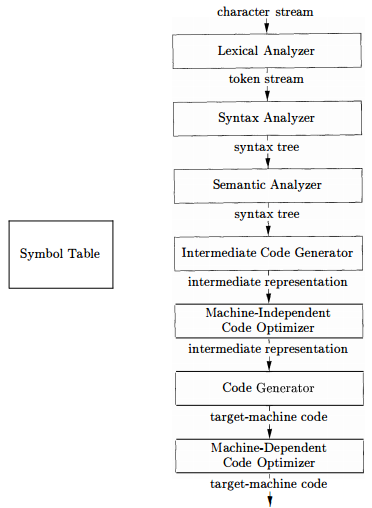
\includegraphics[width=0.7\textwidth]{img/compiler_steps.png}}
    \caption{Traditional steps of a compiler\cite{DragonBook}.}
    \label{fig:compilerSteps}
\end{figure}

\begin{figure}[!htbp]
    \centering
    \begin{tikzpicture}[squarednode/.style={rectangle, draw=black!60, fill=black!5, very thick, 
    minimum width=50mm, minimum height=10mm},]

    \node[](source){source program};
    
    \node[squarednode](lexer)[below=of source]{Lexer};

    \node[](lexemes)[below=of lexer]{Lexemes};
    
    \node[squarednode](parser)[below=of lexemes]{Parser};
    \node[](ast)[below=of parser]{\acro{AST}};

    \node[squarednode](codegen)[below=of ast]{Code Generation};
    
    \node[](html)[below=of codegen]{HTML};

    \node[squarednode](components)[left=of parser]{Component Symbol Table};
    \node[squarednode](variables)[above=of components]{Variable Symbol Table};
    \node[squarednode](functions)[below=of components]{Function Symbol Table};

    \draw[->] (source.south) -- (lexer.north);
    \draw(lexer.south) -- (lexemes.north); 
    \draw[->] (lexemes.south) -- (parser.north); 
    \draw (parser.south) -- (ast.north);
    \draw[->] (ast.south) -- (codegen.north);
    \draw[->] (codegen.south) -- (html.north);


    \end{tikzpicture}
    \caption{Polly's compiler steps \cite{DragonBook}.}
    \label{fig:pollySteps}
\end{figure}



\section{Compiling a template.}
In order to show how \languageName{} compiles a program. It is best shown through a example. The example program is shown in Figure~\ref{fig:sampleProgram}. It is a very simple \textit{``Hello World''} in \languageName{}. All the template is doing is placing a header on the page with ``World'' underlined. First thing that is needed to understand is that Figure~\ref{fig:sampleProgram} is what humans see, with characters hidden for legibility.

\subsection{Lexer}
Firstly the lexer divides each character of the source is then divided into a Iterator(An array of variable length) consisting of tuples(An ordered list of elements) consisting of the character and it's position in the source file.

The \compiler{} keeps track of the characters position in order to provide accurate error messages, showing exactly where the syntax is incorrect. The lexer iterates through the iterator using two functions. \textit{``next()''}, and \textit{``peek()''}. The function \textit{``next()''} takes the next element in the iterator, and advances it's position, so repeatedly calling the function \textit{``next()''} would advance through all the elements. \textit{``peek()''} takes the next element in the iterator, but doesn't advance it's position. So calling \textit{``peek()''}, and then \textit{``next()''} would return the same element.

\begin{figure}[!htbp]
    \begin{verbatim}
        /h1{Hello /u{World}!}
    \end{verbatim}
    \caption{The source of the example.}
    \label{fig:sampleProgram}
\end{figure}

\begin{figure}[!htbp]
    \begin{minted}{rust}
        [
            (0,  '/'), (1,  'h'), (2,  '1'), 
            (3,  '{'), (4,  'H'), (5,  'e'), 
            (6,  'l'), (7,  'l'), (8,  'o'),
            (9,  ' '), (10, '/'), (11, 'u'),
            (12, '{'), (13, 'W'), (14, 'o'),
            (15, 'r'), (16, 'l'), (17, 'd'),
            (18, '}'), (19, '!'), (20, '}')
        ]
    \end{minted}
    \caption{The array of tuples the lexer generates.}
    \label{fig:charIndices}
\end{figure}


The lexer then iterates through tuples, checking each character. If a character is a symbol which is defined in Figure~\ref{fig:lexemes}. It is then parsed into an abstract representation of it using a enum(Enumerated type) see Figure~\ref{fig:lexemes}. If the character is not any of the symbols, the \compiler stores it, and keeps parsing and concatenates all letters into a word.

All whitespace is ignored, and discarded by the lexer, except when there is space around a character, this is to preserve the format of the text. However the lexer will only store one leading, or following space, so \textit{``Hello··World!''} is concatenated to \textit{``Hello·World!''} Both are defined using the \textit{``Lexeme''} enum, which stores the position of the element from the file. See Figure~\ref{fig:lexerOutput} for the output of the Lexer. The lexer's only job is to separate the operators from the words, and provide a slightly more abstract representation of the source file. It doesn't define any logic, or hierarchy.

\begin{figure}
    \begin{minted}{rust}
        pub enum Lexeme {
            Symbol(usize, Operator),
            Word(usize, String),
        }

        pub enum Operator {
            /// The & character used for defining components.
            Ampersand,
            /// The @ character used for defining variables.
            At,
            /// The \ character used for escaping characters.
            BackSlash,
            /// The } character used to singify the end of an 
            /// element.
            CloseBrace,
            /// The ) character used to define the end of a
            /// function call, or attributes list.
            CloseParam,
            /// The , character used to separate arguments 
            /// within a component or function.
            Comma,
            /// The \$ sign used to define a function call.
            Dollar,
            /// The . character used for defining CSS classes
            /// attached to an element.
            Dot,
    \end{minted}
            continued on Figure~\ref{fig:lexemes2}
    \caption{Lexemes for \languageName{}}
    \label{fig:lexemes}
\end{figure}

\begin{figure}
    \begin{minted}{rust}
            /// The = character used for assignment within the
            /// attributes field
            Equals,
            /// The / character used to define elements
            ForwardSlash,
            /// The { character used to signify the start of 
            /// an elements children.
            OpenBrace,
            /// The ( character used to signify the start of 
            /// the attributes for an element, or start of a 
            /// function call
            OpenParam,
            /// The # character used to define CSS ids for an 
            /// element.
            Pound,
            /// The " character used for values within an 
            /// attributes field.
            Quote,
        }
    \end{minted}
    \caption{Lexemes for \languageName{}. Pt.2}
    \label{fig:lexemes2}
\end{figure}

\begin{figure}[!htbp]
    \begin{minted}{rust}
        [
            Symbol(0, ForwardSlash),
            Word(1, "h1"),
            Symbol(2, OpenBrace),
            Word(3, " Hello "),
            Symbol(8, ForwardSlash),
            Word(9, "u"),
            Symbol(10, OpenBrace),
            Word(11, "World"),
            Symbol(16, CloseBrace),
            Word(17, "!"),
            Symbol(18, CloseBrace)
        ]
    \end{minted}
    \caption{Lexer Output.}
    \label{fig:lexerOutput}
\end{figure}



\subsection{Parser}

\subsubsection{Introduction}
The parser takes the output of the lexer, and generates an \acro{AST}. This is where the bulk of the work is done, in terms of determining how the logic is structured, and what the syntax means. The parser has two main contexts, the top level, and the context after certain symbols are defined. The main reason for this is to allow certain operators to have meaning in without requiring \you{} to have to ``escape'' the operators every time they were used. One prime example of this is the \textit{``.''}, or \textit{``Dot''} symbol.

It is used a lot of contexts from being used for \acro{CSS} selectors, and name-spaced identifiers, but if \you{} were writing a paragraph it would be very cumbersome to have to ``escape'' every full stop in a paragraph. So having different contexts allows the syntax, both utilise the \textit{``.''}, for there paragraphs, but also use it with elements for \acro{CSS} class selectors, and to name space variables, and component names.

\begin{figure}[!htbp]
    \begin{minted}{rust}
        pub enum Token {
            Html(Element),
            Text(String),
            Variable(String),
            CompCall(ComponentCall),
            Function(FunctionCall),
        }
    \end{minted}
    \caption{The token enum for the parser.}
    \label{fig:tokenEnum}
\end{figure}

\subsubsection{Text.}
Under the main context, the compiler first checks which lexeme was given. If the lexeme is a \textit{``Word''}, the compiler stores it, and checks if the next lexeme is also a \textit{``Word''}, if it is the compiler then adds it to the previous \textit{``Word''}. The compiler repeats this until the next lexeme isn't a \textit{``Word''}, creating a \textit{``Text''} node, that represents a paragraph.

\textit{``Text''} is a terminal node, meaning that it cannot have any child nodes. Since \textit{``Text''} is purely text, and there is no further logic that can be applied, the positions of each of the words is discarded.

\subsubsection{Variables.}
The next check is to see if the lexeme is a \textit{``@''}, or \textit{``At''} symbol. The \textit{``At''} symbol defines a variable, and the name should map to \acro{JSON} object that is passed to the template. The compiler then takes the next name-spaced identifier.

Where a name-spaced identifier is a a series of lexemes starting with a \textit{``Word''}, and any amount of words providing the previous word was following by a   \textit{``Dot''} symbol e.g. \textit{``@john.doe''}. The \textit{``Variable''} node is also a terminal node. If the next symbol isn't a \textit{``Word''}, the parser will instead provide an error.

\subsubsection{Elements.}
The proceeding check is if the lexeme is a \textit{``/''}, or \textit{``ForwardSlash''} symbol. This is one of the most complex sections of the parser, as during the element definition context, as nearly every symbol has a different meaning. When parsing the element's definition, the compiler takes the first \textit{``Word''}, and defines that as the element's tag, or name e.g. \textit{h1, p, div}. 
\newpage
This identifier cannot be name-spaced, like other nodes, as the  \textit{``Dot''} symbol is used to define a class in the element definition context, and providing it so that at the start of an element's definition, the \textit{``Dot''} symbol has a different use would be unintuitive. 

Within the element definition context, the compiler then checks for the presence of an \textit{``\&''}, or \textit{``Ampersand''} symbol. This defines that instead of having a static body content, the element will instead call this component, optionally with any arguments passed in. The result of the component call, will instead become the body of the element. This means that the element can't also have a static body of text, as it would be confusing for \you{} on where the body of the text would go in the element in relation to the component call's body. This is type of Component call is called a resource.

Since both classes, and id's are the most used html attributes they are given special syntactic sugar in the form of being able to attach CSS selectors. These both take a similar form as the element definition with a \textit{``Dot''} symbol, or \textit{``\#''} or \textit{``Pound''} symbol. Then having the next symbol taken as the name of the class, or id. If it is a \textit{``Word''}, then it is added to the element as a class, or id, if it isn't an error is provided.
Since element attributes are arbitrary, and can take numerous forms, \you{} can also a attach a pair of \textit{``()''}, or \textit{``OpenParam''}, and \textit{``CloseParam''} symbols. Inside these parameter blocks \you{} can define any type of attribute from the traditional key, value pairing e.g. \textit{action=``POST''}, to single word attributes e.g. \textit{``required''}.

All previous symbols can happen in any order after the element definition, so you can have  Class, Id, Class, Resource, Attributes, or Attributes, Resource, Id, Class, Class. To signify the end of defining an element, an \textit{``\{''}, or \textit{``OpenBrace''} symbol. This defines the body of the element. The compiler ignores all lexemes until it finds the appropriate \textit{``\}''}, or \textit{``CloseBrace''}. To do nesting the compiler starts a variable named \textit{``depth''} which starts at zero.
\newpage
As the compiler collects the lexemes, it check if it encounters a \textit{``OpenBrace''}, or \textit{``CloseBrace''}. If the compiler collects a \textit{``OpenBrace''} \textit{``depth''} is incremented by one. If it finds a \textit{``CloseBrace''} \textit{``depth''} is decremented by one. This continues  infinitely until it encounters a \textit{``CloseBrace''}, while \textit{``depth''} is zero. The parser then creates another child parser, and passes the collection of lexemes taken, and attaches the result of this parser to the element.

Additionally, as a form of syntactic sugar if the element ends with attributes, then the braces aren't required for the element. This was designed for \textit{``void''} element e.g. \textit{``meta, link, img''}, but can work for any element.

\subsubsection{Escaping.}
Previously mentioned was how the compiler allows \you{} to be able to have main context symbols used for user facing text. The \textit{``\textbackslash''}, or \textit{``BackSlash''} operator will just convert, the next symbol in the iterator to it's text version, and return a new \textit{``Text''} node containing it.

\subsubsection{Components.}
A component is simply a reusable piece of \languageName{} code. It can also be passed in variables. It does this in a similar way to how it parses the attributes, but instead of key, value pairings. It is is the symbol, plus the name \you{} wants to give the parameter. This parameter is alias, and stored in the component, so \acro{JSON} passed to the parent template, won't poison the component, and provide it values that weren't intended. Components get children in the exact same way as elements.
\newpage
\subsubsection{Functions.}
Unlike Components, and Elements, Functions can't be defined in \languageName{}, so the parser doesn't need to parse the logic of the functions. A \languageName{} function in Rust, takes a reference counted pointer\footnote{A referenced counted pointer, is a data type which tracks the references to it, deallocating when the reference count is zero}, to a reference cell\footnote{A Reference Cell is a data type in Rust, allowing interior mutability, and moving borrow checking to runtime} to the parent template. \verb|Rc<RefCell<Template>>| Functions only take in named arguments, in order to have a cleaner function API in Rust. This works exactly like the attributes in elements.


\begin{figure}[!htbp]
    \centering
    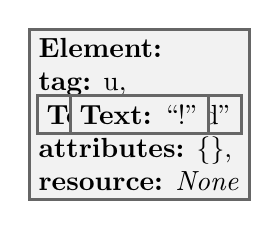
\begin{tikzpicture}[squarednode/.style={rectangle, draw=black!60, fill=black!5, very thick,},]
    \tikzset{level distance=120pt, sibling distance=72pt}
        \Tree[.\node[squarednode, align=left]{
                    \textbf{Element:}\\ 
                    \textbf{tag:} h1,\\
                    \textbf{classes:} [],\\ 
                    \textbf{attributes:} \{\},\\ 
                    \textbf{resource:} \textit{None}}; 
               [.\node[squarednode]{\textbf{Text:} ``Hello''}; ] 
               [.\node[squarednode, align=left]{
                    \textbf{Element:}\\ 
                    \textbf{tag:} u,\\
                    \textbf{classes:} [],\\ 
                    \textbf{attributes:} \{\},\\ 
                    \textbf{resource:} \textit{None}};
                    [.\node[squarednode]{\textbf{Text:} ``World''}; ] ]
               [.\node[squarednode]{\textbf{Text:} ``!''}; ]  ]
    \end{tikzpicture}
    \caption{The \acro{AST} of the example.}
\end{figure}

\subsection{Code Generation.}

Code generation is where the \acro{AST} is converted into the actual desired output, e.g. \acro{HTML}. While this project only focuses on HTML generation, there is no reason in the future the compiler could be expanded to generate other markup languages, such as \acro{XML}. 

Elements are generated first by allocating a String starting with a \textit{``<''}. The elements tag is then added \textit{``<h1''}. The Code generator then checks the elements other properties. If there are any classes they are added, same with attributes. Once that is done a \textit{``>''}, the code generator checks if the element has a resource, or has children, if it has a resource, the code generator calls the component, and creates a new code generator containing the resulting \acro{AST}, and takes that result, appends that to the string. The same is done for direct children, but with the component call Figure~\ref{fig:result}. Components, variables, and Functions are all generated the same way.

\begin{figure}[!htbp]
    \begin{minted}{html}
        <h1>Hello <u>World</u>!</h1>
    \end{minted}
    \caption{The end result.}
    \label{fig:result}
\end{figure}

\subsection{Template}
All of this is provided in a top level API call \textit{``Template''} which stores the functions, components, and \acro{JSON}. The template based on what language passed is passed into the render, will generate the components from the locales files.
\newpage
\section{An advanced example.}
The previous section demonstrated how the compiler works through an example. This section intends to show how the \you{} can actually take advantage of the process of \languageName{}'s compilation steps to perform much more complicated tasks, without compromising on your template by adding complex logic.

One of the most common use-cases for a templating language is to take an array of data that is of unknown length, and format the data into elements. For example a social media website might have a list of friends for a particular user. The website can't know how many every user is going to have, so it has to be designed around the possibility of infinite. See Figure~\ref{fig:websiteTemplate} for the template. It is a relatively simple template, with standard html, the only two new elements are a function call, and a component. The \textit{``std.each''} function takes two named arguments \textit{``array''} \& \textit{``component''}. \textit{``array''} represents the actual array of data to be used, and \textit{``component''} is the template to render for each entry of the array. The component which can simply be described as a reusable section of \acro{HTML}. This component also takes two arguments \textit{``@name''} \& \textit{``@picture''}.

\begin{figure}
    \begin{verbatim}
        /!DOCTYPE(html)
        /html {
            /body {
                /ul#friends-list {
                    $std.each(array = @friends, component = &friend)
                }
            }
        }

        &friend(@name, @picture) {
            /li {
                /img(src=@picture)
                /h4{@name}
            }
        }
    \end{verbatim}
    \caption{Friends list template using function, and components.}
    \label{fig:websiteTemplate}
\end{figure}

\begin{figure}[!htbp]
    \begin{minted}{json}
        {
            "friends": [
                {"name": "Jerry", "picture": "./imgs/jerry.png"},
                {"name": "Elaine", "picture": "./imgs/elaine.png"},
                {"name": "George", "picture": "./imgs/george.png"},
                {"name": "Cosmo", "picture": "./imgs/cosmo.png"}
            ]
        }
    \end{minted}
    \caption{Sample \acro{JSON}.}
    \label{fig:sampleFriends}
\end{figure}
One key steps that is applied to components is that once they are parsed, they are passed into a \textit{``Component Table''} as seen previously in Figure~\ref{fig:pollySteps}. Being placed in a separate table allows for the component to be used regardless of where it was declared as seen in Figure~\ref{fig:websiteTemplate} where the component is is passed to the function before it has been declared. This also allows for importing components, so \you{} can have separate files containing only components and use them in other files. 
\newpage
\subsection{Functions}
Functions behave a lot in the same way as components, but their difference is in the internal logic. Where a component can only generate a very predictable, and partially static html, functions can perform virtually any task as they are defined in Rust, and thusly have access to every library, and every capability Rust has. Functions have full knowledge of the \acro{JSON} that was passed meaning that a function can behave differently  based on types, for example if it was passed an array than if it was passed an object. Functions also have complete access to the component's \acro{AST} meaning it can for example call the component differently based on it's number of arguments.

Both of these features are best shown in the \textit{``std.each''} function. First the function checks if the actual \acro{JSON} was an array, as the function is designed to iterate over an array. The function then checks how many arguments the component that was passed in has. This is where the functions ability inspect it's arguments becomes a very powerful feature. When a component has 0 arguments the function will just generate the component $X$ number of times, where $X$ is the length of the array passed in. When a component has a single argument the items in the array are then passed into that single argument.

The problem arises when there is more than one argument, and for most types of arrays the function will simply provide an error. However the function has a special behaviour for arrays of objects when used with a component with multiple arguments. Instead of simply passing the item to the component the function instead uses the names of the arguments to destructure objects, finding properties with those names. In the example shown previously the \textit{``std.each''} destructures each friend object, and passes the \textit{``name''} \& \textit{``picture''} property of each argument into the \textit{``friend''} component. The objects aren't required to only have those properties, but only properties with the same name as the component argument will be used.

\begin{figure}[!htbp]
    \begin{minted}{html}
    <!DOCTYPE html>
    <html>
    <body>
        <ul>
            <li>
                <img src="./imgs/jerry.png">
                <h4>Jerry</h4>
            </li>
            <li>
                <img src="./imgs/elaine.png">
                <h4>Elaine</h4>
            </li>
            <li>
                <img src="./imgs/george.png">
                <h4>George</h4>
            </li>
            <li>
                <img src="./imgs/cosmo.png">
                <h4>Cosmo</h4>
            </li>
        </ul>    
    </body>
    </html>
    \end{minted}
    \caption{Resulting \acro{HTML}}
    \label{fig:htmlResult}
\end{figure}
  \chapter{Testing}
  \section{Why write tests?}
Writing tests for a \compiler{} is essential, as the smallest changes in behaviour could cause breaking changes in how the \compiler{}, and might break applications using it as a dependency. If \languageName{} was breaking every application that depended on it, developers would be wary of using it. \languageName{} follows \textit{``semver''}(Semantic Versioning)\cite{semver}. Which is concept of having the version number of the program semantically define when API changes occur. For example \languageName{} version X.Y.Z where X means a major version, changes that would break existing programs are signified here.For example if \languageName{} changed the prefix for variables from ``@'' to ``\%'', the major version would be incremented.Y signifies the minor version, which is changes that extend the program, that also don't break existing programs. For example if \languageName{} added another ``std'' function, the minor version would be incremented. Finally Z represents patch versions, which are reserved for backwards-compatible bug fixes. This system allows for users of \languageName{} to know what to expect when developing with \languageName{} and providing a stable, and predictable way to update their dependencies.
\newpage
Tests also provide a helpful tool for developers who want to develop on, and contribute to \languageName{}. As the tests provide an easy way to test if their code should be merged into \languageName{}. If their code fails the tests it can show the developer that their work needs to be improved, before it can merged, or that they need to rewrite current tests if their code makes a breaking change.

\section{Rust's testing framework.}
The testing was done through Rust's built in testing capabilities. In Rust you can test any module by adding an internal module called \textit{``test''} to the file. All functions with the attribute of \textit{``test''} inside the test module will be run, and any functions that complete are considered to have passed the test, and any test that \textit{``panic!''.}'s(An unexpected error, that results in the termination of the thread or program) is considered to have failed. When a test function has failed any errors from the \textit{``panic!''} are printed out to show where the test failed. To allow for easy testing rust has two macros \textit{``assert!''} which takes a boolean and \textit{``panic!''}'s if the value is false and \textit{``assert\_eq!''} which compares two values, and \textit{``panic!''}'s if they aren't equal.
\newpage
\section{\languageName{} testing.}
Due to being a library/\compiler{} tests involving users such as user acceptance testing or usability testing weren't suitable. This is due to the the project having a very niche target, and a high learning curve. As the required knowledge consists of knowledge of \acro{HTML}, \acro{CSS}, the concept of a templating language, and knowledge of Rust. Instead the focus of testing is in types that allow \languageName{} to be a great and stable library/\compiler{}, such as unit tests, end-to-end tests, and regression tests. Performance testing was considered, but due to the lack of pre-existing templating languages built in Rust during the development of \languageName{} there wasn't an opportunity to perform those types of tests.
\subsection{Unit tests.}
Unit testing is one of the smallest form of testing, typically only testing a single module, function, or struct. \languageName{} has most of unit tests on the ``Lexer'' struct. As if the lexer's output isn't what is expected it will have a chain reaction into the parser, and code generation stages which rely on perfect lexer output. Most of the lexer's unit tests are focused on ensuring that certain characters are correctly interpreted as symbols. That unnecessary whitespace is removed, and that when characters are transformed into lexemes that their positions, are the as they were in the source code. Unit tests weren't performed on the parser, or codegen structs, due to the difficulty of replicating the data structures used, as they were designed around being created, and modified through those stages not to be directly instantiated with existing data. See example Figure~\ref{fig:exampleTest}.

\begin{figure}[!hbtp]
    \begin{minted}{rust}
        #[cfg(test)]
        mod test {
            #[test]
            fn dollar_operator() {
                let lexer = Lexer::new("$");

                assert_eq!(lexer.output(), vec![Symbol(0, Dollar)]);
            }
        }
    \end{minted}
    \caption{An example of a test function.}
    \label{fig:exampleTest}
\end{figure}

\newpage
\subsection{End-to-end tests.}
The majority of tests done were end-to-end and regression tests, as these types of tests can encompass much more scope of the program, and accurately inform how the \compiler{} actually compiled a source file. A lot of the tests were written in such a way to actually function as both types of tests. The tests were run using the \textit{``Template''} API as this API is what developers using \languageName{} would use to render their templates. The template API also goes through all the stages of compilation, bubbling up any errors generated. The errors are also written as so that it will clearly differentiate the location of the error, showing if it was from the parser, code generator, or the template itself. On completion of that task without any \textit{``panic!''}'s the end-to-end test is considered a pass.
\newpage
\subsection{Regression tests.}
The output of the end-to-end test is then used in the regression tests, being compared to an expected \acro{HTML} version. There is a version of this type of test for each feature(elements, components, variables, localisation, functions), and also for each ``std'' function provided. These tests provide regression in case any of behaviour change within those features, if the failing test is deemed to be failing due to change(Where the failure is due to intentional behaviour change, and not a bug) the major version of \languageName{} would be incremented, allowing for developer's using the older versions to maintain their code-bases. This also allows developer's to decide when they are comfortable migrating to the latest version.

\begin{figure}[!hbtp]
    \Large{\textbf{Test code(Rust).}}\normalsize{}
    \begin{minted}{rust}
        const BASIC: &'static str = "<!DOCTYPE html><html><body><p>\ 
        Hello World!</p></body></html>";
        #[test]
        fn element() {
            assert_eq!(Template::load("./tests/element.polly")
                           .unwrap()
                           .no_locales()
                           .unwrap_render("en"),
                       BASIC);
        }
    \end{minted}
    \Large{\textbf{Source code(Polly).}}\normalsize{}
    \begin{verbatim}
        /!DOCTYPE(html)
        /html{
            /body {
                /p{Hello World!}
            }
        }
    \end{verbatim}
    \caption{An example of an end-to-end, and regression test.}
\end{figure}
  \chapter{Conclusion}
  This thesis has shown how to build a templating language in Rust. Using extensive research from books such as the \textit{``The Dragon Book''}\cite{DragonBook}, and adapting their core principles into idiomatic Rust code. This thesis has shown the problems of existing templating languages, such as the verboseness of Mustache due to it's need to be usable in any language, and Jade's syntax problem when trying to have layouts, logic, and rich text in a single page. This thesis has shown how \languageName{} address those problems, by removing all forms of explicit logic from the templates, instead moving them to the server's logic.
  \printbibliography
\end{document}